\chapter{Разработка пакета} \label{ch3}

В данной главе рассматривается различные этапы создания пакета. Начиная с разработки и выбора алгоритма работы с ошибками, заканчивая созданием скриптов для создания и удаления пакета.

 
\section{Настройка среды} \label{ch3:sec1}

Для разработки будет использоваться база данных Oracle версии 11g Release 2. Установленная в виртуальную машину Oracle VirtualBox, под управлением ОС Windows Server 2008. Дополнительно нужно установить схемы примеров, предоставляемые Oracle (в дальнейшем потребуется для тестирования), а также пакет UTL\_MAIL для отправки Email сообщений, который поставляется с базой, но не установлен по умолчанию. В качестве среды разработки будем использовать Oracle SqlDeveloper и JetBrains DataGrip. Создадим пользователя, от лица которого будем разрабатывать пакет. 

\begin{figure}[ht!] 
	\center
	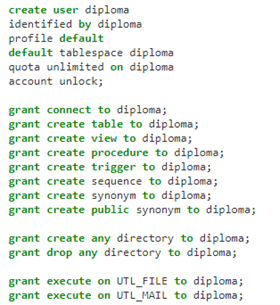
\includegraphics [scale=1] {my_folder/img/C3_create_user.png}
	\caption{Код создания пользователя и выдачи привилегий} 
	\label{fig:C3_create_user}  
\end{figure}
\FloatBarrier

На \firef{fig:C3_create_user} представлен скрипт создания пользователя и выдачи привилегий. Пользователю потребуются: привилегия на создание подключения, создание таблиц, представлений, синонимов и публичных синонимов, последовательностей, процедур и триггеров, привилегии для создания и удаления директорий, а также привилегии на работу с пакетами UTL\_FILE и UTL\_MAIL. 

Данный пользователь предназначен только для разработки, пользователям пакета не нужно будет создавать такого пользователя, поэтому использование некоторых потенциально опасных привилегий (например, drop any directory) является допустимым. Если в ходе разработки потребуются дополнительные разрешения, об этом будет специально указано.


\section{Структура распространяемого пакета} \label{ch3:sec2}

Пакет будет распространяться как SQL скрипт, который состоит из установщика и скриптов самого пакета. Инсталлер выполняет работу по созданию основных объектов, таблиц, триггеров, последовательностей, представлений. После чего производится вставка данных, в основные таблицы, сюда входит информация о базовых ошибках, описание их типов, создание параметров и выставление их в значения по умолчанию. Так же установочный скрипт занимается созданием директории для логирования файлов.


\section{Схема хранения информации} \label{ch3:sec3}

Первоначально, для решения проблемы работы с кодами ошибок, необходимо сокрыть их использование за процедурами пакета. Опишем сущность исключительной ситуации, с которой будем работать в дальнейшем. 

Для ошибки нам необходимо хранить следующую информацию: код ошибки, наименование ошибки, тип ошибки и информацию о ней, а также дополнительную мета информацию, в которую будет входить, временная метка создания записи об ошибки, и имя пользователя, который создал данную ошибку. Номер ошибки (код) будет использоваться в ходе работы пакета, для упрощения идентификации, пользователи же будут использовать наименования ошибки, так как правильно выбранное имя, более подробно описывает суть ошибки и проще для запоминания человеком, но, в случае необходимости, пользователи все также могут обращаться к ошибкам по кодам. Это позволит сделать разрабатываемый пакет расширяемым, не скрывая от пользователей всех возможностей. 

Данная информация будет храниться в таблице ERRM\$ERRORS, которая будет связана с таблицей ERRM\$ERROR\_TYPES. Таблица ERRM\$ERROR\_TYPES будет содержать описание типов исключительных ситуаций. Типы позволят разделить ошибки на группы, и обрабатывать ошибки по-разному в зависимости от их важности. Информация, хранящаяся о категориях, подобна той информации, которую мы храним об ошибках, здесь содержится ID типа, наименование типа и информация о нем. 

Модель хранения данных, используемая в пакете, представлена на \firef{fig:C3_er_model}.

\begin{figure}[ht!] 
	\center
	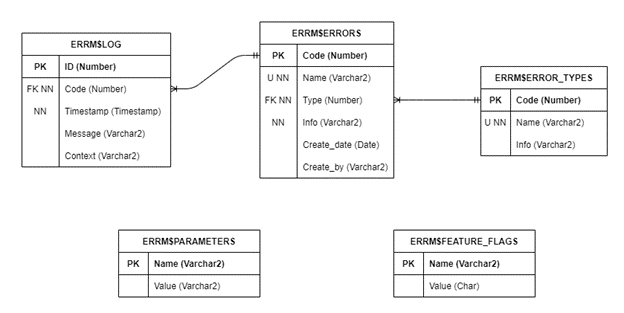
\includegraphics [scale=1] {my_folder/img/C3_er_model.png}
	\caption{ER модель хранения информации пакета} 
	\label{fig:C3_er_model}  
\end{figure}
\FloatBarrier

Здесь и далее, для Entity-relationship моделей используются следующие обозначения: PK – первичный ключ (Primary Key), FK – внешний ключ (Foreign Key), U – уникальное поле (Unique), NN – обязательное поле (Not null). 

Таблица ERRM\$ERRORS имеет ссылочное ограничение на первичный ключ таблицы ERRM\$ERROR\_TYPES. 
Возникающие в ходе работы приложения, ошибки необходимо хранить для дальнейшего анализа, для данных целей присутствует таблица ERRM\$LOG, в которую заносится номер записи, код ошибки (имеется связь с таблицей ERRM\$ERRORS), временная метка возникновения ошибки, сообщение, а также контекст данной ситуации. 

Здесь, и в дальнейшем, под контекстом ошибки понимается набор именованный набор данных, если не сказано иного.  

Дополнительно, присутствуют две таблицы для задания параметров пакета, это ERRM\$PARAMETERS и ERRM\$FEATURE\_FLAGS. Вторая таблица хранит установленные значения опций, то есть тех настроек, которые имеют бинарное значение (включена/выключена), например возможность логирования информации в файл. А первая отвечает за настройку не бинарных параметров, например, название файла для записи информации об ошибках, почта администратора. 


\section{Дополнительные объекты для обработки информации} \label{ch3:sec4}
 
Помимо перечисленных в параграфе \ref{ch3:sec3} таблиц, нам необходимы дополнительные объекты базы данных, которые будут обеспечивать целостность и корректность хранимой информации.

Первая категория - это последовательности. Последовательность – это объект базы данных, предоставляющий пользователю последовательность чисел по указанным правилам. Нами будет использоваться три последовательности. Первая – для кода ошибок, вторая – для номера типов ошибок, и третья – для последовательного номера записи в таблице логирования.  

Во вторую категорию попадают триггеры на таблицы. Для таблиц ERRM\$PARAMETERS и ERRM\$FEATURE\_FLAGS за счет триггеров будет контролироваться вид хранимой информации, все имена параметров должны храниться в верхнем регистре, а значения параметров - в нижнем, значения для feature flag должны быть либо символом 0, либо символом 1. В случае, если пользователи будут добавлять некорректные данные, триггер не позволит вставить такую информацию, обновление информации будет отклонено, возникнет исключение с сообщением. 


\section{Определение спецификации пакета} \label{ch3:sec5}
 
Весь пакет (спецификация и тело) будет образно разделен на подкатегории, таким образом пользователям будет проще ориентироваться в пакете, читаемость кода такого пакета будет выше. Были выделены следующие категории структуры пакета: 

\begin{enumerate} 
\item CONSTANTS – в данном блоке будут объявляться константные значения пакета
\item TYPES – объявление используемых типов данных
\item PARAMETERS WORK – процедуры и функции для настройки параметров пакета
\item HELPERS – дополнительные действия 
\item PROCEDURE AND FUNCTIONS – методы для основной работы с пакетом
\item SILENT RAISES – методы для вызова исключений без логирования
\item LOG WORK – процедуры работы с местами хранения логов
\item SIMPLE ERROR RAISE – процедуры для упрощения вызова часто используемых ошибок
\item LOG – блок для вывода информации на экран, упрощение работы с пакетом DBMS\_OUTPUT
\end{enumerate} 

В коде пакета данные категории будут помечены комментариями и разделяться пустыми строками. Данное разделение является условным и на работу программы не влияет. 

Выделим типы, с которыми будем работать. Объявив типы (или подтипы, как в нашем случае) мы сможем отвязаться от конкретного способа хранения данных, и, в случае, когда тип нужно будет изменить, например если код ошибки потребуется хранить не числом, а строкой, это сделать будет очень просто, поменяв объявление типа в спецификации пакета. Мною были объявлены следующие типы данных:

\begin{enumerate} 
\item t\_err\_code – тип для идентификации ошибки, является подтипом типа pls\_integer 
\item t\_err\_name – тип для работы с именем ошибки, подтип varchar2 размером в 100 символов.
\item t\_err\_type – тип для хранения категории ошибки, наследуется от типа pls\_integer
\end{enumerate} 

Для возможности настройки параметров пакета нам потребуется, как минимум, 4 метода. Получение и задания значений параметров, а также получений и задание флагов возможностей. Оба метода на получение установленного значения будут принимать один входной параметр – имя настройки, а возвращать сохраненное в таблице значение, отличие будет в возвращаемом типе данных, для параметров это будет строка (varchar2), для опций это Boolean. 

Так же для работы с опциями и параметрами объявим несколько строковых констант, в которых будут сохранены имена для параметров. Это позволит пользователям не заботиться о правильности написания названия того или иного параметра, а просто обратиться к константе. 

Для констант будут использоваться следующие префиксы: FEATURE\_ для бинарных опция (которые хранятся в таблице ERRM\$FEATURE\_FLAGS, подробнее смотри в параграфе \ref{ch3:sec3}) и PARAMETER\_, собственно, для параметров (хранятся в таблице ERRM\$PARAMETERS). При помощи этих префиксов будет понятно, какие методы нужно использовать, и какое значение мы ожидаем в результате работы функции. 

\begin{figure}[ht!] 
	\center
	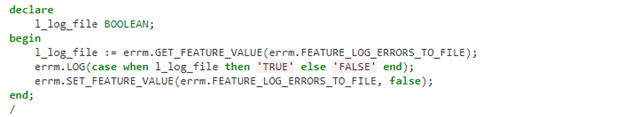
\includegraphics [scale=1] {my_folder/img/C3_get_feature.png}
	\caption{Пример получения и установки значения опции} 
	\label{fig:C3_get_feature}  
\end{figure}
\FloatBarrier

На \firef{fig:C3_get_feature} показан пример использования описанных ранее процедуры и функции для работы с опциями. В данном анонимном блоке объявляется бинарная переменная, в которую заносится значение опции FEATURE\_LOG\_ERRORS\_TO\_FILE, которая отвечает за логирование в файл. После чего происходит вывод информации на экран, при помощи метода LOG (о нем будет сказано далее), затем происходит отключение возможности логирования в файл.

Использование констант также защищает пользователей от дополнительных ошибок, если бы пользователю пришлось задавать название параметра вручную, велика вероятность опечатки, и в результате мы получим ошибку на этапе исполнения, когда программа сделает запрос к таблице и не найдет параметра с таким значением. В случае же использования констант среда разработки подскажет, какие константы мы можем использовать, но даже в случае опечатки, ошибка возникнет еще на этапе компиляции, что позволит заметить ее гораздо раньше, и исправить. При этом функции GET\_FEATURE\_VALUE и GET\_PARAMETER\_VALUE принимают строки, что дает возможность пользователям, в случае необходимости, обратиться к значениям настроек на прямую, без использования констант. 

Методы для вывода информации из категории LOG, сюда входит две процедуры LOG (которая уже использовалась ранее) и NL. Данные методы являются обертками для вызовов стандартных методов из пакета DBMS\_OUTPUT. Процедура LOG работает аналогично, процедуре PUT\_LINE, а процедура NL скрывает за собой процедуру NEW\_LINE. Это упрощает написание кода для отладки, и позволяет с легкостью заменить вывод отладки, например, на вывод в файл, достаточно будет поправить только один метод. Нет нужды заставлять пользователей использовать данные методы, так как не известно как конкретно работает логирование в пользовательском приложении, довольно вероятна ситуация, когда используется другой пакет, например, log4plsql (популярный фреймворк для логирования информации, предоставляет множество различных мест логирования, поддерживает Oracle Forms, Oracle Report\cite{log4plsql}), но для удобства они были вынесены в спецификацию.

В категорию HELPERS входит единственный метод GET\_ERROR\_CODE, который позволяет по имени ошибки получить ее код. Методы для пользователей имеют определения как для работы с кодами ошибок, так и для работы с именами ошибок (что является более предпочтительным), но данная функциональность может потребоваться пользователям пакета. Допустим, что имеется необходимость не вызывать ошибку прямо сейчас, а требуется записать ошибку, либо передать ее куда-то, выполнить дополнительную работу (собрать расширенный контекст ошибки), и только потом вызвать исключение, в таком случае можно сохранить (или передать в другой метод) имя ошибки, в котором произойдет необходимая работа, после чего, при помощи данного метода происходит получение кода ошибки, проводятся дополнительные операции с ошибкой, и в итоге происходит вызов ошибки. Суммируя, данная функциональность расширяет перечень возможностей пакета. 

Рассмотрим процедуры для работы с местами логирования информации (категория LOG WORK). Сюда включены две процедуры CLEAR\_LOG\_TABLE и CLEAR\_LOG\_FILE. Как понятно из их названия, они предназначены для очистки хранилища ошибок, таблицы или файла, соответственно. 

Далее будут рассмотрены методы для основной работы с пакетом. 

Процедура REGISTER\_ERROR предназначена для создания ошибки, за ней будет скрываться вставка данных в таблицу ERRM\$ERRORS, предваренная дополнительными действиями, генерация кода ошибки, если он не указан, приведение имени ошибки к стандартному имени и так далее. На вход процедура принимает: код ошибки, не обязательный параметр, наименование ошибки (обязательно), тип ошибки (не обязательно, по умолчанию устанавливается обычная ошибка), информация об ошибке (обязательно), комментарий про использование данного вида ошибки. Информация об ошибке фактически не является обязательным параметром, но будем обязывать пользователей ее указывать, чтобы при возникновении ошибки была максимально понятна ее суть. Поля с датой создания и именем пользователя-создателем, будут обновляться при помощи триггера. 
Для вызова ошибки будут использоваться методы RAISE, всего таких методов будет 4. Первый (самый предпочтительный вариант) принимает в параметрах имя вызываемой ошибки, и не обязательный флаг p\_log\_enabled, который отвечает за необходимость логирования информации об ошибке. Второй метод, принимает вместо имени код ошибки, имеет аналогичный второй параметр. В обоих этих методах параметр p\_log\_enabled не является обязательным и по умолчанию имеет значение true, что означает, что логирование будет производиться. 

Остальные два метода имеют префикс s (сокращение от слова silent(англ.) – тихий), итоговое название SRAISE, они вызывают обычный метод raise, с установкой второго параметра в значение false. Что означает, что логирование производиться не будет. Данный обработчик используется в тех случаях, когда нужно прервать выполнение программы, но не требуется заносить информацию об этом. Данные методы, по умолчанию, принимают имя ошибки в качестве параметра, но имеет перегрузку процедуры, в которой задается номер ошибки, вместо имени. 

В категорию SIMPLE ERROR RAISE попадают процедуры, которые позволят вызвать исключение одной строчкой, не нужно знать даже наименование ошибки, что очень удобно для часто используемых исключительных ситуаций. В данный момент, сюда включено 4 метода, для заранее предопределенных ошибок: DEFAULT\_ERROR, DEFAULT\_LOG, DEFAULT\_WARNING и NOT\_IMPLEMENTED\_EXCEPTION. Первые три представляют собой вызов стандартных (для данного пакета) исключительных ситуаций с разными типами (подробнее смотри в параграфе \ref{ch3:sec3}), последний является вызовом ошибки, которая гласит, что код еще не реализован. 

Рассмотрим пример, пользователь разрабатывает пакет, определил спецификацию и реализовал в теле не все методы, но имеется желание уже протестировать работу данных процедур и/или функций. Для нереализованных методов можно создать простую реализацию с заглушкой состоящей из одной команды null, которая не выполняет никаких действий, но такая ситуация является опасной, если метод так и не будет реализован, то при вызове этих методов ничего не произойдет, проблема заключается в том, что об этом никто не узнает, пользователь, вызывая код на исполнение, ожидает, что метод выполнит свою работу, но этого не происходит. Если же использовать исключение, то при вызове данного метода, сразу станет понятно, что метод еще не готов, и использовать его еще рано. Так же это упростит процедуру автоматического тестирования, так как нам будет сразу известно, что метод не выполнил работу, и нам нет нужды производить более сложную проверку. 

Рассмотрим, как будет проходить взаимодействие пользователей с контекстом ошибок. Для этого в пакете предусмотрены две процедуры ADD\_CONTEXT и CLEAR\_CONTEXT. Первая добавит к контексту дополнительную информацию, принимает два строковых параметра: название и значение. Вторая очищает значения в сохраненном контексте. Контекст автоматически очистится после вызова ошибки.

\begin{figure}[ht!] 
	\center
	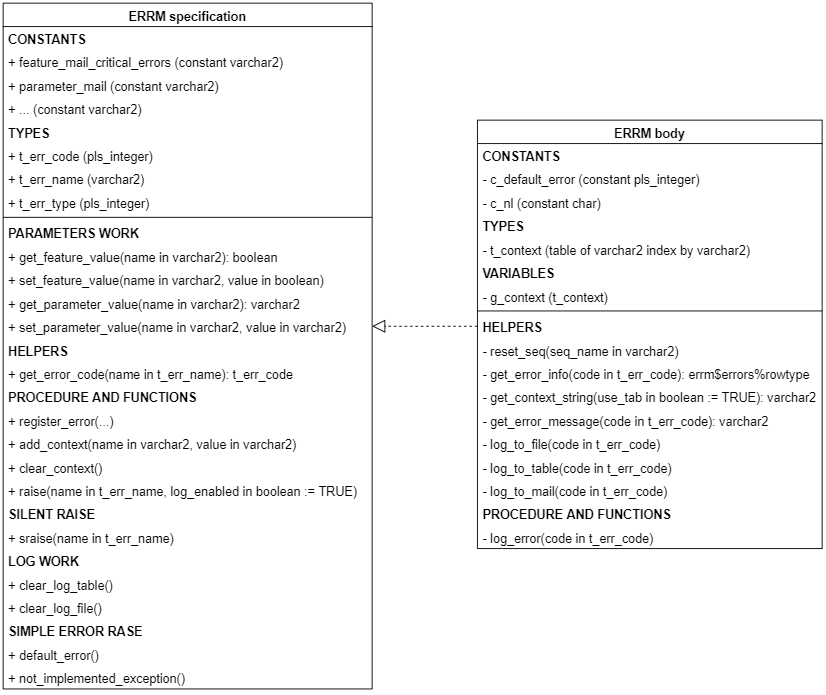
\includegraphics [scale=0.6] {my_folder/img/C3_UML_diagram.png}
	\caption{UML диаграмма пакета} 
	\label{fig:C3_UML_diagram}  
\end{figure}
\FloatBarrier

На \firef{fig:C3_UML_diagram} представлена схематичная UML диаграмма пакета, на ней показаны не все, а только основные процедуры и функции. В теле пакета указаны только методы, отличные от спецификации пакета, остальные методы, тоже будут реализованы. Категории блоков пакета выделены жирным. 


\section{Создание установщика} \label{ch3:sec6}

Весь пакет состоит из четырех файлов: установщик, определение спецификации пакета, определение тела пакета, деинсталлер. Установщик занимается созданием и настройкой необходимых объектов, после чего запускает скрипты для создания пакета. В итоге три первых скрипта могут быть объединены в один, для исключения лишних ошибок. 

Рассмотрим принципиально важные моменты создания установщика. Все начинается с создания таблицы типов ошибок ERRM\$ERROR\_TYPES. Код этой части инсталлера представлен на  \firef{fig:C3_create_error_types_table}.

\begin{figure}[ht!] 
	\center
	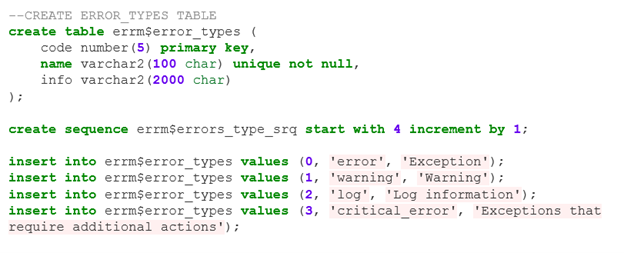
\includegraphics [scale=1] {my_folder/img/C3_create_error_types_table.png}
	\caption{Код создания таблицы типов} 
	\label{fig:C3_create_error_types_table}  
\end{figure}
\FloatBarrier

Первоначально создается таблица для хранения типа ошибок, затем создается последовательность для хранения кодов типов, после чего производится вставка нескольких базовых типов. 

\begin{figure}[ht!] 
	\center
	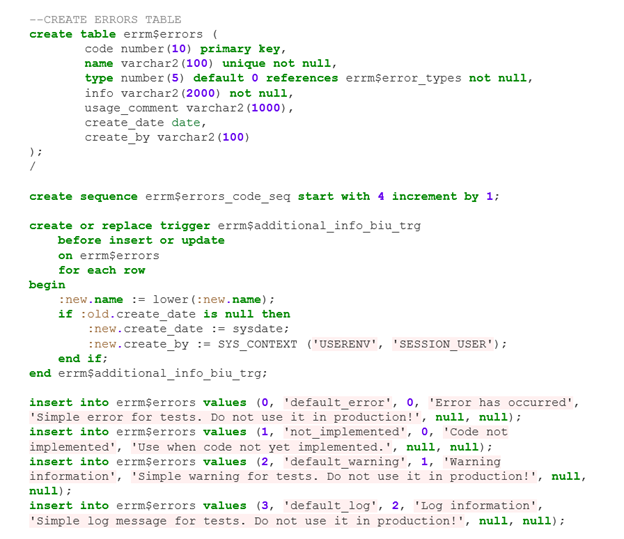
\includegraphics [scale=1] {my_folder/img/c3_create_errrors_table.png}
	\caption{Код создания таблицы ошибок} 
	\label{fig:c3_create_errrors_table}  
\end{figure}
\FloatBarrier

На \firef{fig:c3_create_errrors_table} представлен код создания таблицы ошибок, создания последовательности. 

Создается триггер, который приводит имя ошибки к стандартному виду и добавляет мета информацию при создании новой записи. Для этого используется стандартная процедура SYS\_CONTEXT, которая позволяет получить имя пользователя. 

\begin{figure}[ht!] 
	\center
	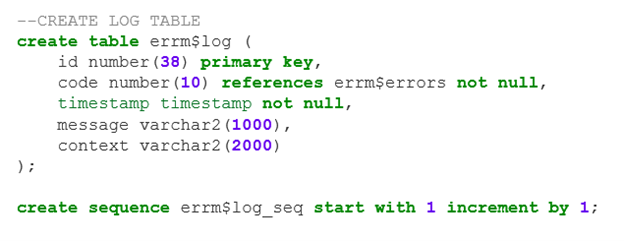
\includegraphics [scale=1] {my_folder/img/C3_create_log_table.png}
	\caption{Код создания таблицы для логирования} 
	\label{fig:C3_create_log_table}  
\end{figure}
\FloatBarrier

На \firef{fig:C3_create_log_table} показан код создания таблицы для хранения логов ошибки, и последовательности, для нумерации логов.

Код для создания остальных таблиц ERRM\$PREFERENCES и ERRM\$FEATURE\_FLAGS, а также триггеров и данных, можно посмотреть в приложении \ref{appendix-1}. 


\section{Разработка тела пакета} \label{ch3:sec7}

Далее будут подробно описаны принципиально важные участки пакета, менее важные моменты рассмотрены не будут, полный код пакета содержится в приложении \ref{appendix-1}.

Схематичный алгоритм вызова исключения представлен на \firef{fig:c3_block_diagram}. 

\begin{figure}[ht!] 
	\center
	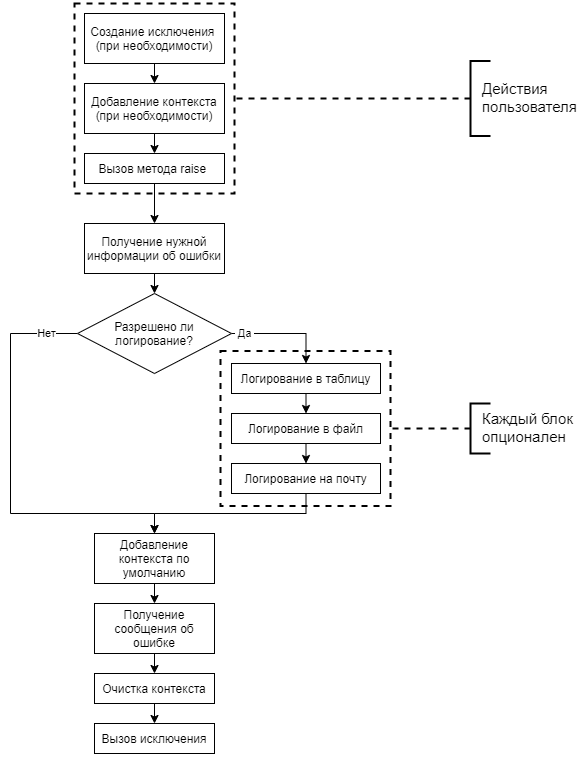
\includegraphics [scale=1] {my_folder/img/c3_block_schema.png}
	\caption{Блок схема вызова исключения} 
	\label{fig:c3_block_diagram}  
\end{figure}
\FloatBarrier

Первые операции (выделенные в блок) выполняет пользователь, остальное скрыто за реализацией пакета. В случае логирования информации об ошибке, каждая процедура для логирования информации в определенное место (например, на почту), проверяет доступность этого метода согласно установленным значениям опций пакета. 

Вызов исключения всегда происходит с определенным кодом, который задается при создании тела пакета, используется значение -20000, зарезервированное Oracle для пользовательских приложений. Данное значение вынесено в константу, при необходимости использовать другой код, пользователи могут заменить номер в теле пакета. Вызов исключения происходит при помощи стандартной процедуры RAISE\_APPLICATION\_ERROR, в которую передается указанный код, а также отформатированное сообщение об ошибке, в нем указывается название и код исключительной ситуации из пакета, краткое описание ошибки, тип ошибки и контекст. В случае, если включено все логирование эта же информация заносится в таблицу ERRM\$LOG, и в файл логирования. Если возникшая ошибка является критической, происходит отправка письма администратору, почта которого задается в параметрах пакета. 

Данное описание справедливо для процедуры RAISE принимающей код ошибки. 

Все остальные методы для возбуждения исключения (RAISE с именем ошибки, два вида SRAISE, упрощенные методы для вызовы часто используемых ошибок) сводятся к вызову основного метода RAISE.

\begin{figure}[ht!] 
	\center
	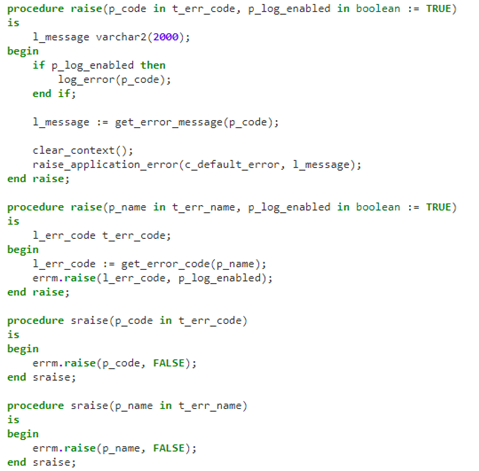
\includegraphics [scale=1] {my_folder/img/c3_raise_code.png}
	\caption{Код метода Raise} 
	\label{fig:c3_raise_code}  
\end{figure}
\FloatBarrier

Код процедуры RAISE и того, как остальные процедуры завязаны на основной метод представлен на \firef{fig:c3_raise_code}. 

Методы для упрощенного вызова ошибок работают следующим образом: вызывается метод RAISE c указанным в методе кодом ошибки. Для расширения перечня таких методов пользователи могут добавить аналогичные методы, либо в данный пакет и перекомпилировать его, либо в какое-либо свое пространство. Данное действие рекомендуется провести для всех часто используемых ошибок. 

Для логирования информации об ошибке основной метод RAISE вызывает процедуру LOG\_ERROR. Которая, в свою очередь, вызывает три процедуры, каждая из который заносит информацию об ошибке, в свое место. 

\begin{figure}[ht!] 
	\center
	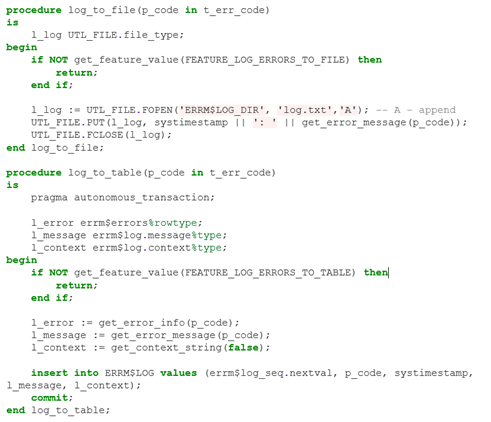
\includegraphics [scale=1] {my_folder/img/c3_log_to_file_code.png}
	\caption{Коды процедур логирования в файл и в таблицу} 
	\label{fig:c3_log_to_file_code}  
\end{figure}
\FloatBarrier

На \firef{fig:c3_log_to_file_code} представлены процедуры для занесения информации в файл и в таблицу, соответственно. Каждая процедура перед логированием информации, проверяет включена ли соответствующая опция. Метод LOG\_TO\_FILE открывает файл при помощи функции UTL\_FILE.FOPEN, с параметром A, который позволяет добавить информацию в конец файла и заносит необходимую информацию. 

Метод LOG\_TO\_TABLE получает необходимые значения, сюда входит: номер лога, сообщение об ошибке, контекст ошибки, а затем вносит данные в таблицу. Метод объявлен как автономная транзакция, это необходимо для того, чтобы данные в таблице ERRM\$LOG не откатились вместе с основной транзакцией при возникновении ошибки (которая будет далее вызвана методом RAISE).

\begin{figure}[ht!] 
	\center
	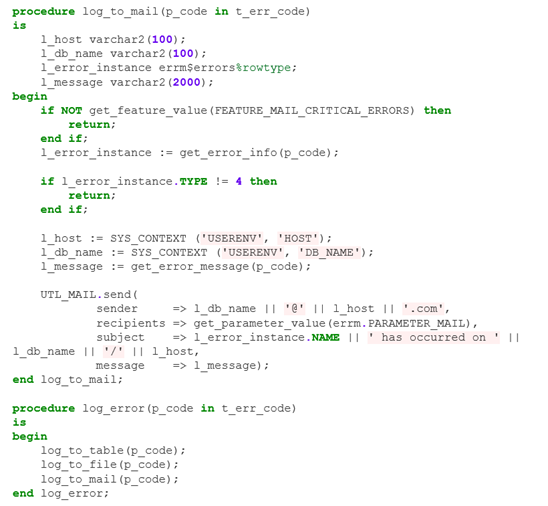
\includegraphics [scale=1] {my_folder/img/c3_log_code.png}
	\caption{Код логирования ошибок} 
	\label{fig:c3_log_code}  
\end{figure}
\FloatBarrier

Код, представленный на \firef{fig:c3_log_code} отвечает за логирование критических ошибок на почту, и общий метод логирования, который и вызывает процедура RAISE. Процедура LOG\_TO\_MAIL, отправляет письмо администратору, адрес которого указывается в параметрах приложения. 

Процедура LOG\_ERROR по очереди вызывает ранее описанные методы. 

Очистка мест сбора информации происходит следующим образом. В случае хранения информации в файле (метод CLEAR\_LOG\_FILE), файл открывается для записи, при помощи пакета UTL\_FILES, функцией FOPEN, с указанием параметра W, что очистит файл для записи новой информации. После чего файл сразу же закрывается. В результате данного действия файл станет пустым. 

Сложнее происходит очистка таблицы ERRM\$LOG, помимо удаления данных из самой таблицы, необходимо обнулить последовательность номеров лога. Пересоздать последовательность заново мы не можем, так как, в этом случае пакет (имеющий зависимость на эту последовательность) потребует перекомпиляции. Обнулять последовательность будем способом, показанным на \firef{fig:c3_clear_code}. 

\begin{figure}[ht!] 
	\center
	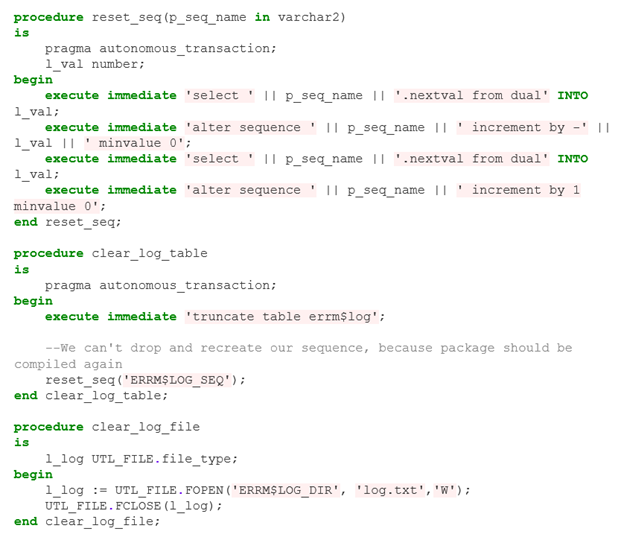
\includegraphics [scale=1] {my_folder/img/c3_clear_code.png}
	\caption{Код процедур для очистки мест логирования} 
	\label{fig:c3_clear_code}  
\end{figure}
\FloatBarrier

Здесь представлен фрагмент кода с очисткой файла логирования, и метод для очистки таблицы логирования. Сама очистка таблицы происходит посредством вызова динамического SQL кода, а конкретно команды TRUNCATE TABLE, после чего происходит вызов процедуры RESET\_SEQ, в который передается имя последовательности. 
В методе RESET\_SEQ происходит динамический вызов четырех команд SQL. Первоначально из последовательности извлекается следующее число, далее происходит изменение последовательности при помощи команды ALTER SEQUENCE, изменяется шаг на отрицательное значение, полученного на прошлом этапе числа. Далее извлекается следующее значение последовательности, в результате чего текущее число последовательности обнулится. Последняя команда возвращает шаг последовательности к начальному значению. 


\section{Работа с контекстом} \label{ch3:sec8}

Для сохранения контекста ошибки будет использоваться схема, описанная далее. В теле пакета объявляется тип данных t\_context, являющийся таблицей, хранящей тип varchar2 и индексируемой типом varchar2 (аналог ассоциативного массива в PL/SQL, еще называемый словарем). А также объект данного типа с именем g\_context. При помощи метода ADD\_CONTEXT, в данный словарь будут вноситься данные. При возникновении ошибки информация из контекста попадает в лог, ассоциативный массив очищается, для хранения контекста новых ошибок. Процедура CLEAR\_CONTEXT позволяет очищать контекст вручную, в случае необходимости. 
Дополнительная процедура ADD\_DEFAULT\_CONTEXT добавляет к контексту системную информацию, в нее включены: наименование экземпляра, обслуживающего базу, наименование базы данных, имя пользователя, имя приложения из которого выполнялась работа, текущая схема, наименование хоста. Описанный базовый контекст может добавляться автоматически, ко всем возникшим ошибкам, это поведение настраивается флагом в таблице ERRM\$FEATURE\_FLAGS, по умолчанию включено.  

\begin{figure}[ht!] 
	\center
	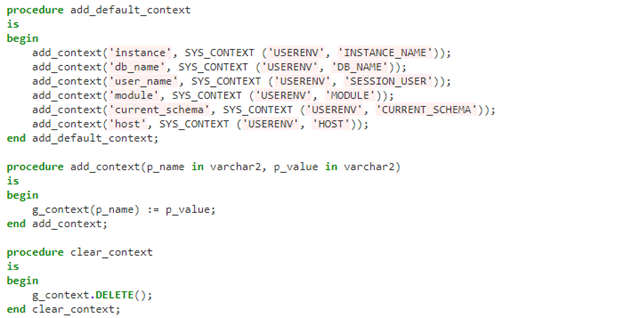
\includegraphics [scale=1] {my_folder/img/c3_add_context_code.png}
	\caption{Методы добавления информации в контекст ошибки} 
	\label{fig:c3_add_context_code}  
\end{figure}
\FloatBarrier

На фрагменте кода, представленном на \firef{fig:c3_add_context_code}, показаны методы для добавления контекста, для очистки словаря контекста, и для заполнения словаря контекстом по умолчанию. 

Так же для работы с контекстом, используется метод GET\_CONTEXT\_STRING, который формирует из словаря строку с информацией о хранящихся в контексте данных, которая в дальнейшем добавляется в лог. Код данной функции представлен на \firef{fig:c3_get_context_code}.


\begin{figure}[ht!] 
	\center
	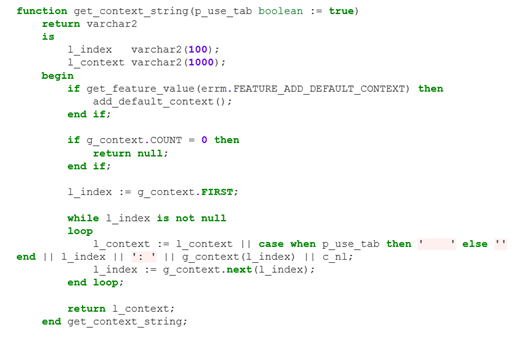
\includegraphics [scale=1] {my_folder/img/c3_get_context_code.png}
	\caption{Функция получения строки контекста} 
	\label{fig:c3_get_context_code}  
\end{figure}
\FloatBarrier

Добавление контекста по умолчанию, происходит именно в этом методе, так как строка с контекстом обязательно будет запрошено при вызове исключения. В качестве параметра, данная функция принимает флаг, указывающий нужно добавлять дополнительный отступ перед параметрами контекста, для логирования в таблицу данный отступ не является необходимым, потому что контекст будет храниться в отдельном столбце, а для вывода на экран и в файл, отступ будет упрощать чтение сообщения об ошибке.

Данный подход для работы с контекстом почти не ограничивает пользователя в хранимом количестве данных, ограничение появляется только при достижении лимита размера типа varchar2. Максимальный размер данного типа 4000 байт, что эквивалентно 4000 символов в одно байтовой кодировке или 2000 символов в двухбайтовой. Данного объема обычно достаточно для ошибок, контекст ошибки не должен содержать больших данных, но при этом должен давать максимально подробное описание ситуации. В дальнейшем, при необходимости, можно реализовать альтернативный механизм хранения контекста, который не подвержен данному ограничению, например, большой контекст помещать в файл, а в основном контексте оставлять ссылку на файл. 

\section{Отчеты об ошибках} \label{ch3:sec9}
 
Были создали два представления для получения информации о популярных ошибках и о самых часто встречающихся. 

\begin{figure}[ht!] 
	\center
	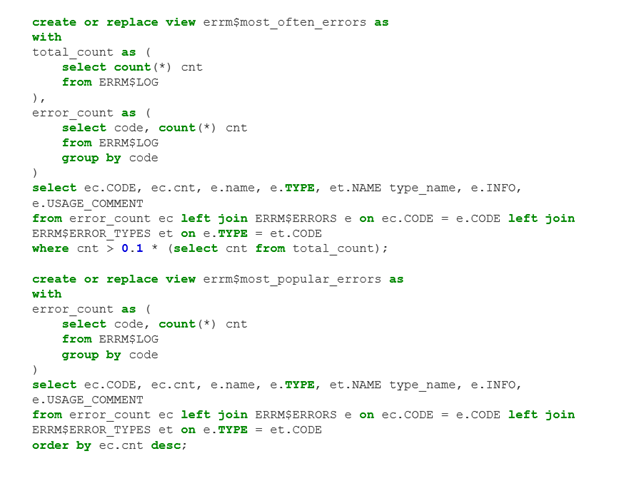
\includegraphics [scale=1] {my_folder/img/c3_view_code.png}
	\caption{Создание представлений} 
	\label{fig:c3_view_code}  
\end{figure}
\FloatBarrier

Код на \firef{fig:c3_view_code}, показывает, как создаются указанные представления. 
В представлении ERRM\$MOST\_OFTEN\_ERRORS содержится информация о тех ошибках, что встречаются чаще 10\% от общего числа сохраненных ошибок. 
Представление ERRM\$MOST\_POPULAR\_ERRORS содержит список всех возникших ошибок, отсортированный по количеству появлений. 


\section{Удаление пакета} \label{ch3:sec10}

Для удаления пакета из системы был разработан скрипт, в котором реализована правильная последовательность удаления объектов пакета. 

\begin{figure}[ht!] 
	\center
	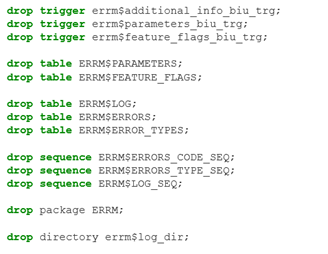
\includegraphics [scale=1] {my_folder/img/c3_uninstall.png}
	\caption{Скрипт удаления пакета} 
	\label{fig:c3_uninstall}  
\end{figure}
\FloatBarrier

На \firef{fig:c3_uninstall} представлен данный скрипт. В первую очередь удалим триггеры. Далее необходимо удалить объекты в обратной последовательности от их создания. Сначала удаляются таблицы, не имеющие зависимостей, затем происходит удаление таблиц, на которые не ссылаются другие таблицы (изначально существует только одна такая таблица это ERRM\$LOG, поэтому она удаляется первой, затем таблица ERRM\$ERRORS не имеет таблиц, ссылающихся на нее, и может быть удалена), и далее по цепочке. Затем удаляются созданные во время установки последовательности. В последнюю очередь удаляется сам пакет и директория для логирования.
Полный код пакета, и всех остальных скриптов можно посмотреть в приложении \ref{appendix-1}. 


\section{Выводы} \label{ch3:conclusion}


В данной главе был разработан пакет для работы с ошибками, были созданы скрипты для установки и удаления данного пакета, разобраны основные методы пакета. Рассмотрены алгоритмы сохранения информации об ошибках. 


%% Вспомогательные команды - Additional commands
%
\newpage % принудительное начало с новой страницы, использовать только в конце раздела
%\clearpage % осуществляется пакетом <<placeins>> в пределах секций
%\newpage\leavevmode\thispagestyle{empty}\newpage % 100 % начало новой страницы